\documentclass{article}
\usepackage[utf8]{inputenc}

\title{Report.3.OpenMP.tex}
\author{gw.muraro }
\date{30 October 2018}

\usepackage{natbib}
\usepackage{graphicx}
\usepackage{pgfplots}

\begin{document}

\maketitle
\section{Labwork 3}
\subsection{Explain how you implement the labwork}

    The work is in few steps : 
    \begin{enumerate}
        \item Set the variables of the number of pixel, by getting height and width of the image to convert, the number of blocks and their sizes :
        \begin{verbatim}
        int pixelCount = inputImage->width * inputImage->height;
        int blockSize = 1024;
        int numBlock = pixelCount/blockSize ;
        \end{verbatim}
        
        \item Allocate 2 arrays on the GPU's memory with the pixel number using cudaMalloc :
        \begin{verbatim}
        uchar3 * devInput ;
        uchar3 * devGray ;

        cudaMalloc(&devInput, pixelCount * sizeof(uchar3));
        cudaMalloc(&devGray, pixelCount * sizeof(uchar3));    
        \end{verbatim}
        
        
        \item Copy the memory from the CPU to the GPU using cudaMemcpy and precising we go from the host to the device. 
        \begin{verbatim}
        cudaMemcpy(devInput, inputImage->buffer, pixelCount * sizeof(uchar3), cudaMemcpyHostToDevice);
        \end{verbatim}
        
        
        \item Launch the kernel 
        \begin{verbatim}
        grayScale<<<numBlock, blockSize>>>(devInput, devGray) ;
        \end{verbatim}
        
        The kernel looks like that
        \begin{verbatim}
        __global__ void grayScale(uchar3 *input, uchar3 *output) {
                int tid = threadIdx.x + blockIdx.x * blockDim.x;
                output[tid].x = (input[tid].x + input[tid].y + input[tid].z) / 3;
                output[tid].z = output[tid].y = output[tid].x;
        }
    
        \end{verbatim}
        
        \item Copy the memory from the GPU to the output variable (in CPU)
        \begin{verbatim}
        cudaMemcpy(devGray, outputImage, pixelCount * sizeof(uchar3), cudaMemcpyDeviceToHost);
        \end{verbatim}
        
        \item Do not forget to free malloc-ed variables
        \begin{verbatim}
        cudaFree(devInput);
        cudaFree(devGray);
        \end{verbatim}
    
    \end{enumerate}
    
\subsection{What’s the speedup?}
    
    \begin{verbatim}
        # labwork 1
        [...]
        labwork 1 CPU ellapsed 3724.7ms
        labwork with pragmas ellapsed 805.3ms
        
        
        # labwork 3
        [...]
        labwork 3 ellapsed 77.6ms
    \end{verbatim}
    
    Comparing with the single processor program, we divided by ~48 times the computing time. 
    Comparing with the CPU-parralelized program, we divided by ~10 times the computing time. 
    
\subsection{Plot a graph of block size vs speedup}
    A new program argument has been added in order to gain time for block size tests. See the source code for further informations. 
    \newline
    At least we got these results :
    \newline
    %%plot
    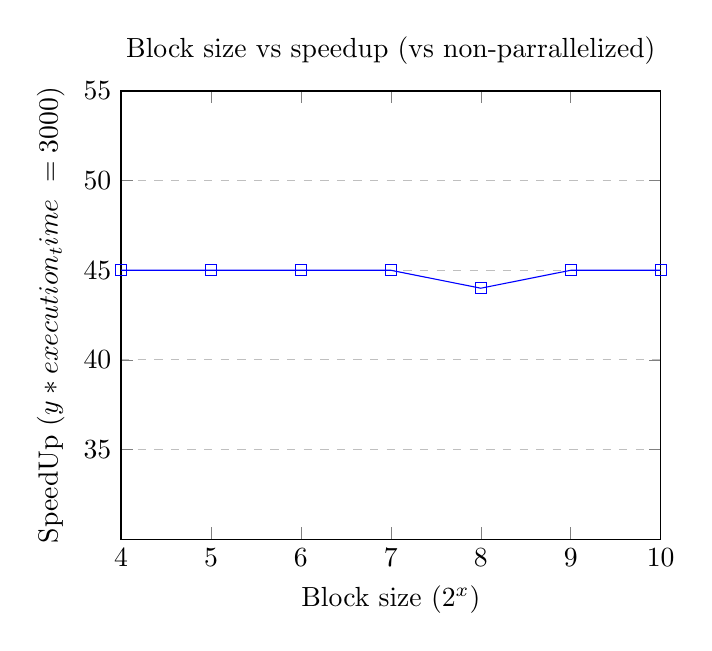
\begin{tikzpicture}
        \centering
        %%define axes
        \begin{axis}[
            title={Block size vs speedup (vs non-parrallelized)},
            xlabel={Block size ($2^x$)},
            ylabel={SpeedUp ($y*execution_time ~= 3000$)},
            xmin=4, xmax=10,
            ymin=30, ymax=55,
            xtick={4,5,6,7,8,9,10},
            ytick={35, 40, 45, 50, 55},
            legend pos=north west,
            ymajorgrids=true,
            grid style=dashed,
        ]
        %% data filing
        \addplot[
            color=blue,
            mark=square,
            ]
            coordinates { %% Remind : axis X = 2^x
                (4, 45)(5,45)(6,45)(7,45)(8,44)(9,45)(10,45)
            };

        \end{axis}
    \end{tikzpicture}
    \newline
    We can see that there is not much difference between the number of block used and the speed up (always around 45 times faster than the non paralleled program).
    However, it is important to note that the image was black on output, and it size was small compared to the base image. 
    
\end{document}

